\chapter{CRIStAL laboratory}

\section{History}

CRIStAL\footnotemark[1]\cite{cristal} (Research Center in Computer Science, Signal and Automatic Control of Lille), founded on the 1\st of January 2015, is a laboratory of CNRS\footnotemark[2] (National Center for Scientific Research), Lille 1 university and Centrale Lille in partnership with Lille 3 University, Inria (French National Institute for computer science and applied mathematics) and Mines Telecom Institute. It is the result of the fusion of LAGIS\footnotemark[4] (Laboratory of Automatic Control, Computer Engineering and Signal) and LIFL\footnotemark[4] (Laboratory of Fundamental Computing of Lille) to federate their complementary competencies in information sciences. It is a member the interdisciplinary research institute IRCICA\footnotemark[5] (Research Institute on Software and Hardware Components for Advanced Information and Communication in Lille). \\

\footnotetext[1]{``Centre de Recherche en Informatique, Signal et Automatique de Lille''}

\footnotetext[2]{``Centre national de la recherche scientifique''}

\footnotetext[3]{``Laboratoire d'Automatique, G\'enie Informatique et Signal''}

\footnotetext[4]{``Laboratoire d'Informatique Fondamentale de Lille''}

\footnotetext[5]{``Institut de recherche sur les composants logiciels et mat\'eriels pour l'information et la communication avanc\'ee de Lille''}

CRIStAL is located in Villeneuve d'Ascq city in Lille, the capital of  the Hauts-de-France region and the prefecture of the Nord department and the fourth largest urban area in France after Paris, Lyon and Marseille. Chaired by \textit{Prof.Olivier Colot}, it harbours about 430 personnel with exactly 228 permanents and more than 200 non-permanents. Permanent researchers are divided among more than 30 teams working on different themes and projects.

\begin{figure}[!ht]
	\centering
	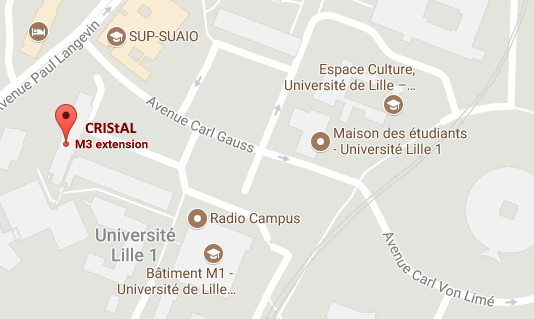
\includegraphics[scale=0.4 , frame]{img/cristalLocation.png} 
	\caption{CRIStAL laboratory Location}
\end{figure}

%reference annex organigram + add cristal to image

\section{Research activities}

CRIStAL's research activities concern topics related to the major scientific and societal issues of the moment such as: Big Data, software, computer imaging, human-machine interactions, robotics, control and supervision of large systems, intelligent embedded systems, bioinformatics\dots The laboratory is involved in the development of revolutionary platforms such as Pharo, a pure object oriented language and a powerful yet simple development environment used worldwide.

\section{2XS team}

The 2XS (eXtra Small, eXtra Safe) team is working on highly constrained embedded devices, precisely on designing software and hardware that are secure, safe and efficient. Research in this team is focused on defining new system architectures or new languages to allow fast development of reliable embedded software. The team addresses issues concerning memory footprint, energy consumption and security and takes profit from proficiencies in formal verification, hardware/software co-design and operating system architectures to tackle the aforementioned issues.\\

The team is lead by \textit{Prof.Gilles Grimaud} and has 15 members\footnotemark[1] as well as several trainees and most of its current work mainly revolves around the PIP project and its applications.

\begin{figure}[!ht]
	\centering 
	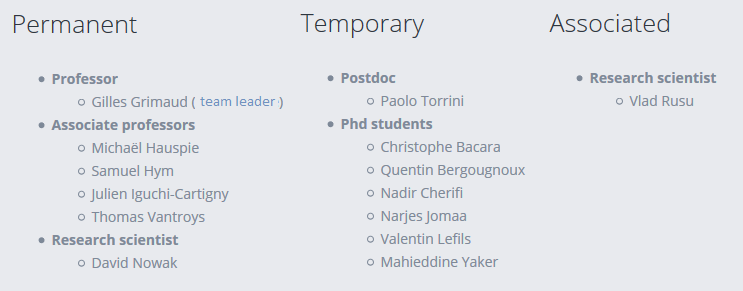
\includegraphics[width=\linewidth, frame]{img/2XS.png} 
	\caption[The 2XS team organizational chart]{The 2XS team organizational chart\cite{cristal}}
\end{figure}

% reference to PIP project section

\footnotetext[1]{as of \today}



